\section{mo\-SA$<$ M $>$ Class Template Reference}
\label{classmo_s_a}\index{moSA@{moSA}}
Simulated Annealing (SA).  


{\tt \#include $<$mo\-SA.h$>$}

Inheritance diagram for mo\-SA$<$ M $>$::\begin{figure}[H]
\begin{center}
\leavevmode
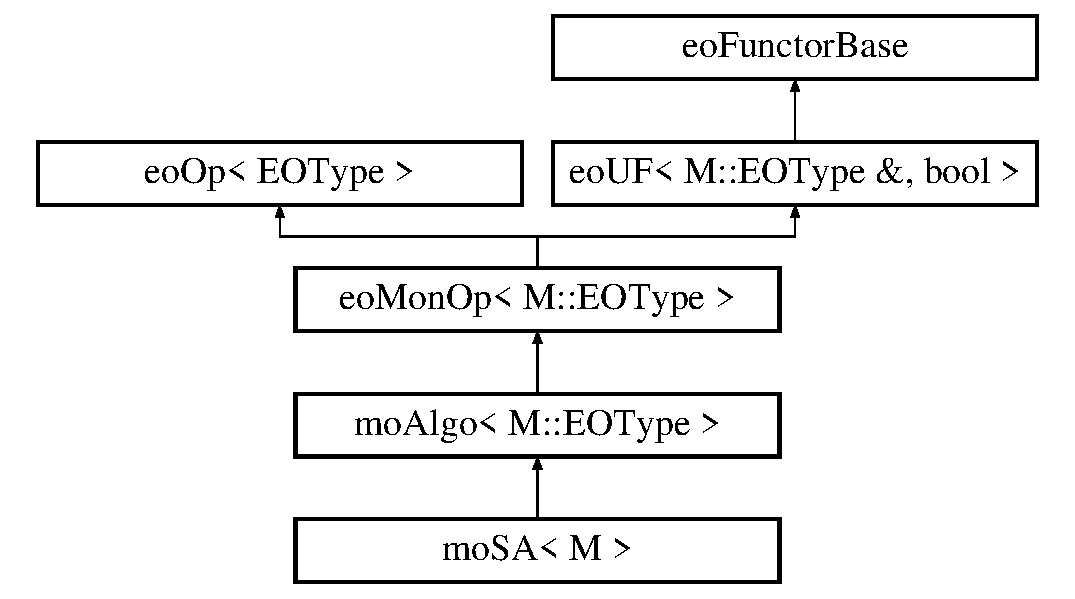
\includegraphics[height=2cm]{classmo_s_a}
\end{center}
\end{figure}
\subsection*{Public Member Functions}
\begin{CompactItemize}
\item 
{\bf mo\-SA} ({\bf mo\-Rand\-Move}$<$ M $>$ \&\_\-\_\-move\_\-rand, {\bf mo\-Move\-Incr\-Eval}$<$ M $>$ \&\_\-\_\-incr\_\-eval, {\bf mo\-Sol\-Continue}$<$ {\bf EOT} $>$ \&\_\-\_\-cont, double \_\-\_\-init\_\-temp, {\bf mo\-Cool\-Sched} \&\_\-\_\-cool\_\-sched, eo\-Eval\-Func$<$ {\bf EOT} $>$ \&\_\-\_\-full\_\-eval)
\begin{CompactList}\small\item\em SA constructor. \item\end{CompactList}\item 
bool {\bf operator()} ({\bf EOT} \&\_\-\_\-sol)
\begin{CompactList}\small\item\em function that launches the SA algorithm. \item\end{CompactList}\end{CompactItemize}
\subsection*{Private Types}
\begin{CompactItemize}
\item 
typedef M::EOType {\bf EOT}\label{classmo_s_a_d5d64a8797bdedc7b3af7893aded0bd5}

\begin{CompactList}\small\item\em Alias for the type. \item\end{CompactList}\item 
typedef EOT::Fitness {\bf Fitness}\label{classmo_s_a_97f1a40d5ab5a0b3f878d0347b34804b}

\begin{CompactList}\small\item\em Alias for the fitness. \item\end{CompactList}\end{CompactItemize}
\subsection*{Private Attributes}
\begin{CompactItemize}
\item 
{\bf mo\-Rand\-Move}$<$ M $>$ \& {\bf move\_\-rand}\label{classmo_s_a_71c49935b63a202d25888a5f86121fec}

\begin{CompactList}\small\item\em A move generator (generally randomly). \item\end{CompactList}\item 
{\bf mo\-Move\-Incr\-Eval}$<$ M $>$ \& {\bf incr\_\-eval}\label{classmo_s_a_4c3be32e9832e465b24e6d33559356bc}

\begin{CompactList}\small\item\em A (generally) efficient evaluation function. \item\end{CompactList}\item 
{\bf mo\-Sol\-Continue}$<$ {\bf EOT} $>$ \& {\bf cont}\label{classmo_s_a_54484c8a514866ea496e0058c2e09716}

\begin{CompactList}\small\item\em Stopping criterion before temperature update. \item\end{CompactList}\item 
double {\bf init\_\-temp}\label{classmo_s_a_f1af7636b52aa5f6b381f8187b667bd4}

\begin{CompactList}\small\item\em Initial temperature. \item\end{CompactList}\item 
{\bf mo\-Cool\-Sched} \& {\bf cool\_\-sched}\label{classmo_s_a_c7aaf7424aa1b9f889d2ba9c959e5a1d}

\begin{CompactList}\small\item\em The cooling schedule. \item\end{CompactList}\item 
eo\-Eval\-Func$<$ {\bf EOT} $>$ \& {\bf full\_\-eval}\label{classmo_s_a_bcd6a940046f23dd741444c0b85edf2c}

\begin{CompactList}\small\item\em A full evaluation function. \item\end{CompactList}\end{CompactItemize}


\subsection{Detailed Description}
\subsubsection*{template$<$class M$>$ class mo\-SA$<$ M $>$}

Simulated Annealing (SA). 

Class that describes a Simulated Annealing algorithm. 



Definition at line 32 of file mo\-SA.h.

\subsection{Constructor \& Destructor Documentation}
\index{moSA@{mo\-SA}!moSA@{moSA}}
\index{moSA@{moSA}!moSA@{mo\-SA}}
\subsubsection{\setlength{\rightskip}{0pt plus 5cm}template$<$class M$>$ {\bf mo\-SA}$<$ M $>$::{\bf mo\-SA} ({\bf mo\-Rand\-Move}$<$ M $>$ \& {\em \_\-\_\-move\_\-rand}, {\bf mo\-Move\-Incr\-Eval}$<$ M $>$ \& {\em \_\-\_\-incr\_\-eval}, {\bf mo\-Sol\-Continue}$<$ {\bf EOT} $>$ \& {\em \_\-\_\-cont}, double {\em \_\-\_\-init\_\-temp}, {\bf mo\-Cool\-Sched} \& {\em \_\-\_\-cool\_\-sched}, eo\-Eval\-Func$<$ {\bf EOT} $>$ \& {\em \_\-\_\-full\_\-eval})\hspace{0.3cm}{\tt  [inline]}}\label{classmo_s_a_ef9ffb0d95c599e0a06c78db5f2f4b12}


SA constructor. 

All the boxes used by a SA need to be given.

\begin{Desc}
\item[Parameters:]
\begin{description}
\item[{\em \_\-\_\-move\_\-rand}]a move generator (generally randomly). \item[{\em \_\-\_\-incr\_\-eval}]a (generaly) efficient evaluation function \item[{\em \_\-\_\-cont}]a stopping criterion. \item[{\em \_\-\_\-init\_\-temp}]the initial temperature. \item[{\em \_\-\_\-cool\_\-sched}]a cooling schedule, describes how the temperature is modified. \item[{\em \_\-\_\-full\_\-eval}]a full evaluation function. \end{description}
\end{Desc}


Definition at line 60 of file mo\-SA.h.

\subsection{Member Function Documentation}
\index{moSA@{mo\-SA}!operator()@{operator()}}
\index{operator()@{operator()}!moSA@{mo\-SA}}
\subsubsection{\setlength{\rightskip}{0pt plus 5cm}template$<$class M$>$ bool {\bf mo\-SA}$<$ M $>$::operator() ({\bf EOT} \& {\em \_\-\_\-sol})\hspace{0.3cm}{\tt  [inline]}}\label{classmo_s_a_0e4c54b57bc13fcbd4763883b8f719e5}


function that launches the SA algorithm. 

As a {\bf mo\-TS}{\rm (p.\,\pageref{classmo_t_s})} or a {\bf mo\-HC}{\rm (p.\,\pageref{classmo_h_c})}, the SA can be used for HYBRIDATION in an evolutionary algorithm.

\begin{Desc}
\item[Parameters:]
\begin{description}
\item[{\em \_\-\_\-sol}]a solution to improve. \end{description}
\end{Desc}
\begin{Desc}
\item[Returns:]TRUE. \end{Desc}


Definition at line 82 of file mo\-SA.h.

References mo\-SA$<$ M $>$::full\_\-eval.

The documentation for this class was generated from the following file:\begin{CompactItemize}
\item 
mo\-SA.h\end{CompactItemize}
